\section{Floquetifying the colour code}\label{sec:floquetifying_colour_code}

We can apply the same ideas as in the last section to stabilizer codes
more interesting than the $\qcode{4, 2, 2}$ code.
In this section, we take this more interesting stabilizer code to be the colour code (\Cref{ex:colour_code_stabilizer_code}).
Recall that the colour code can be defined on both a planar surface and any closed surface, like the torus.
%Or, more accurately, we take it to be the \textit{bulk} of the colour code -
%i.e.\ ignoring the code's global topology (whether it lives on a torus, or is planar).
%A discussion of global topology is deferred to
%\Cref{subsec:floquetifying_colour_code_beyond_bulk} at the end of this section,
%and continued in detail in \Cref{sec:floquetifying_colour_code_beyond_bulk}.

\subsection{The colour code bulk}\label{subsec:floquetifying_colour_code_bulk}
%
%The $\mathit{6.6.6}$ \textit{colour code} is a stabilizer code defined on a honeycomb lattice, with qubits placed at vertices.
%We write $v \in f$ to mean that a vertex $v$ is incident to a hexagonal face $f$.
%For any such face $f$, we define weight-six Paulis $X_f = \prod_{v \in f} X_v$ and $Z_f = \prod_{v \in f} Z_v$.
%On a torus, the code is defined by the measurement schedule
%$\MMM = [\langle \{Z_f: \text{face $f$}\} \rangle,~ \langle \{X_f: \text{face $f$}\} \rangle]$.
%On a planar geometry, slightly different Paulis are measured at the boundaries~\cite{ColourCodeBoundariesAndTwists}.

\begin{figure}[t]
    \centering
    
\includegraphics[width=\linewidth]{figures/qubits/floquetifying/colour_code/zx_rewritten}
    \caption{
        Two equivalent ZX-diagrams for a patch of the colour code at three consecutive timesteps.
        Ideally we'd draw vertical wires connecting each column of patches,
        like we were able to do for the $\qcode{4, 2, 2}$ code in the last section,
        but doing this renders the diagrams pretty much unreadable.
        Instead, we draw very small vertical wires going up and/or down from certain spiders, labelled by letters.
        These letters define how a wire going vertically upwards in one layer is actually connected to
        a wire coming vertically downwards from the layer above it;
        wires labelled by the same letter are connected.
    }
    \label{fig:colour_code_rewritten}
\end{figure}

As before, we start with a ZX-diagram of the colour code over multiple timesteps;
see the left hand side of \Cref{fig:colour_code_rewritten}.
Maybe more accurately, we start with a subdiagram of the colour code in the \textit{bulk} (away from any boundaries, if this colour code is planar).
By `tiling' copies of this subdiagram, we can create larger and larger subdiagrams of colour code bulk.
So if we can reason about this subdiagram we can reason about the whole bulk.

We then unfuse every spider into four or five spiders to get the diagram on the right of the figure.
In these diagrams, grey hexagons, bars and integers, as well as letter labels and coloured wires, all have no meaning in the ZX-calculus; they're just visual aids.
In the diagram on the right, wires within grey bars correspond to weight-two measurements,
while all other wires correspond to qubit world-lines.
The focus is on a single qubit's world-line, which we've coloured purple;
we can see that it's only involved in measurements with four other qubits,
which we've coloured orange, pink, blue and brown.
It turns out that all qubit world-lines have this property of only interacting with four other qubits.
Furthermore, these interactions are such that the qubits of the new code can be laid out on a square lattice.
So henceforth we'll label qubits of the new code with a pair of integer coordinates $(x, y)$.

The grey bars labelled by integers denote the timesteps of the new code.
These are well-defined;
picking any qubit world-line and following it up the page
while noting down the integer label of every grey bar it crosses produces an increasing sequence.
For example, doing this for the purple qubit produces the contiguous sequence $(0, 1, 2, \ldots)$.
As before, we can view all one-legged spiders as halves of single-qubit measurements.
The pattern repeats after every two timesteps of the old code (the colour code);
one can see this by noting that the bottom and top of the diagram are identical,
up to a translation in space and an increase by 13 in the labels of the grey bars.
%In other words, this new code has a period of 13.

\begin{figure}[t]
    \centering
    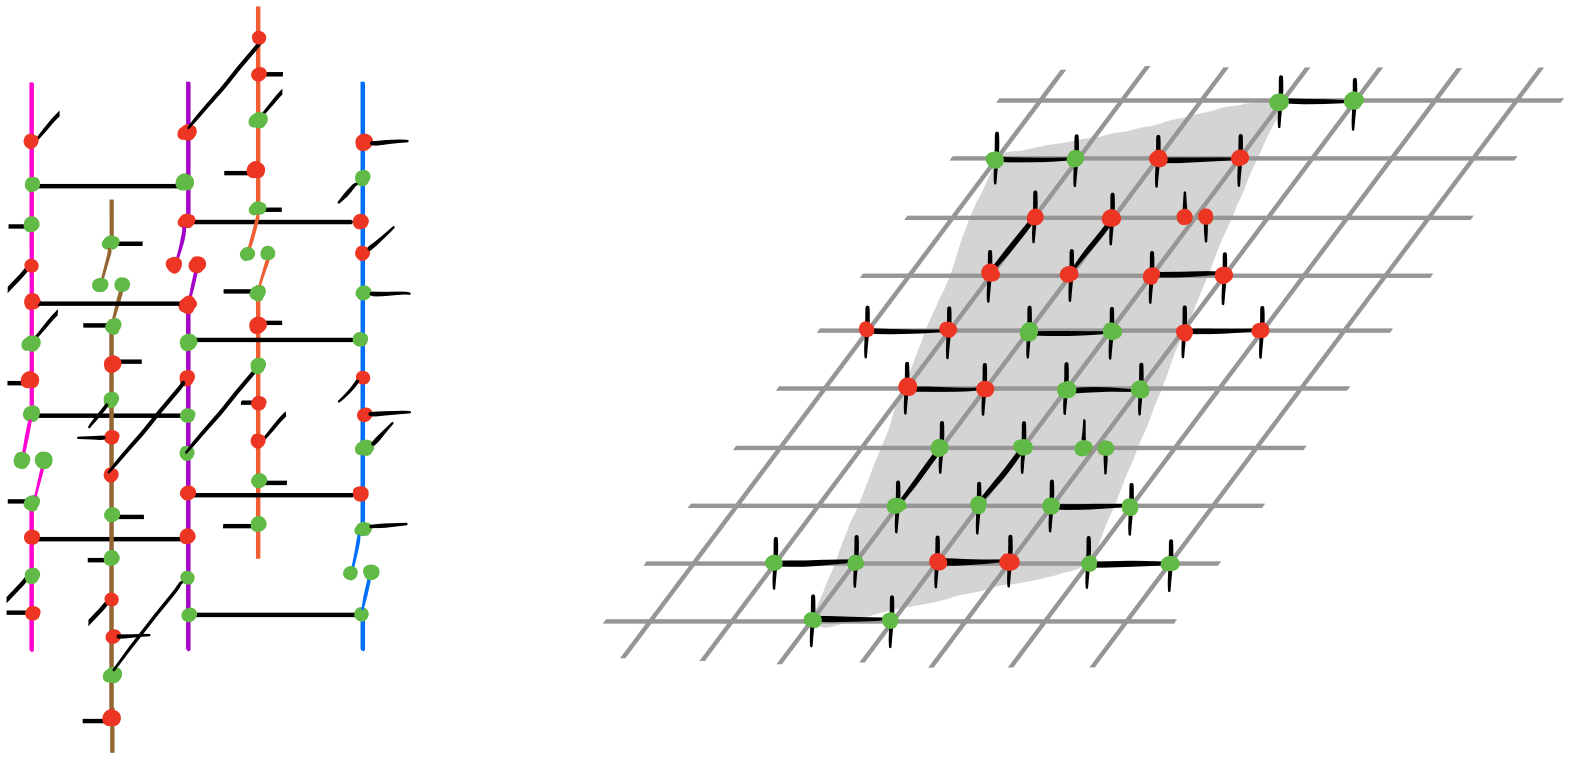
\includegraphics[width=\linewidth]{figures/qubits/floquetifying/colour_code/floquetified/measurement_schedule}
    \caption{
        Left: measurements undergone by a single qubit and its four nearest neighbours over one full period of 13 timesteps.
        Right: One `tile' of one timestep of the measurement schedule in the bulk of the Floquetified colour code.
        Here the grey lines are \textit{not} ZX-diagram wires -
        they are just visual aids that show this all sits on a square lattice.}
    \label{fig:floquetified_colour_code_measurement_schedule}
\end{figure}

Again, we can now write down the measurements that each qubit undergoes at each timestep.
In \Cref{fig:floquetified_colour_code_measurement_schedule},
we show a ZX-diagram of this, focused on the purple qubit from \Cref{fig:colour_code_rewritten}.
Each qubit undergoes essentially the same pattern of measurements in each period.
Specifically, whatever measurement qubit $(x, y)$ undergoes at timestep $t$,
qubit $(x, y+1)$ undergoes it at time $t-2$, but with the roles of $Z$ and $X$ exchanged.
Likewise for the remaining neighbours $(x+1, y)$, $(x, y-1)$ and $(x-1, y)$,
but at times $t-8$, $t+2$ and $t+8$ respectively.

Knowing all this, we can then write down the operation sequence (i.e.\ measurements) for the bulk of a potential new Floquetified version of the colour code.
This has a periodic structure; we draw a ZX-diagram for a single timestep $t$ and single `tile' of this on the right of \Cref{fig:floquetified_colour_code_measurement_schedule}.
To see the measurements happening across the whole bulk at this timestep, one should tile these grey rectangles across the square lattice.
That is, whatever measurement qubit $(x, y)$ undergoes at time $t$, qubits $(x+3, y+1)$ and $(x-2, y+8)$ undergo this too.
Then to get the measurements happening at the next timestep, one should translate the measurements from time $t$ by $(-1, -3)$.
That is, whatever measurement qubit $(x, y)$ undergoes at time $t$, qubit $(x-1, y-3)$ undergoes it at time $t+1$.
\begin{figure}[t]
    \centering
    
\includegraphics[width=\linewidth]{figures/qubits/floquetifying/colour_code/floquetified/detector}
    \caption{
        A detecting region in the colour code and the corresponding detecting region in the Floquetification.
        Again, grey lines are \textit{not} ZX-diagram wires -
        they are just a visual guide showing the square lattice.}
    \label{fig:detector_floquetified_colour_code}
\end{figure}

As in the last section, Pauli webs in the original diagram have an image in the new diagram.
In \Cref{fig:detector_floquetified_colour_code} we show a detecting web in the colour code bulk and its image in the bulk of the potential new Floquet code.
The corresponding detector in the potential new code consists of 14 weight-two measurements and 4 single-qubit measurements, spread over 8 timesteps.
Every detector in the bulk of the potential new code is identical to this one, up to a space-time translation and exchanging $Z$ and $X$.
%Just as in the colour code, one can show these detecting webs are tiled such that unique errors
%violate unique sets of detectors, so decoding can be performed,
%though we leave investigating specific decoding strategies to future work.
A similar exercise can be repeated for the logical webs;
one can draw the logical webs corresponding to the known logical operators of the colour code,
one can see how the (known!) logical webs in the colour code map to logical webs in the Floquetified code,
from which one can write down the support in the bulk of the potential new code's logical operators.

This process raises questions, however (as might be clear from the fact I keep saying `potential' new code).
If this is to be the bulk of a new Floquet code, will there be boundaries?
If so, what will the operation sequence there look like, given that the operation sequence at the boundaries of the colour code is slightly different to that of the bulk?
If not, i.e.\ we instead implement this potential new Floquet code on a closed surface like a torus, is it still fair to say we have Floquetified the original code?
In the next subsection, we discuss both of these possible routes to finishing off our Floquetification.

\subsection{Beyond the bulk: periodic boundaries}\label{subsec:floquetifying_colour_code_beyond_bulk}

Let's start with the scenario where the code we wish to Floquetify has periodic boundaries, e.g.\ it lives on a torus.
In \Cref{eq:timeslice_4_2_2_double_hexagon} in the last section, we said that we can interpret our Floquetification procedure as tilting the time direction in a ZX-diagram.
If we attempt to do this for a code with periodic boundary conditions,
this tilting can have the effect of `making time run circularly'.
%\jm{\sout{fancy! But for a proper (topological) code with a threshold you want to define a code family such that you effectively take the limit of all directions to infinity (before or after floqueification, these two operations should commute). So even then the time-periodicity wouldn't matter, right? For finite-size codes this can be problem, I see that.}}
The diagram below illustrates the problem:
a `thickened' torus $T^2 \times I$ is shown in blue
(faces of the cube marked with the same letters $A$ and $B$ are glued together),
and three planes through it are drawn in different shades of grey.
The thickened torus is an abstraction for a ZX-diagram showing the time evolution of a code that lives on a torus,
while the three grey planes are potential new timeslices after Floquetifying this code.
However, it's impossible to label these three planes with unique integers
such that a line perpendicular to them passes through them an increasing sequence:
\begin{equation}\label{eq:toric_spacetime_volume_timeslice}
\begin{aligned}
    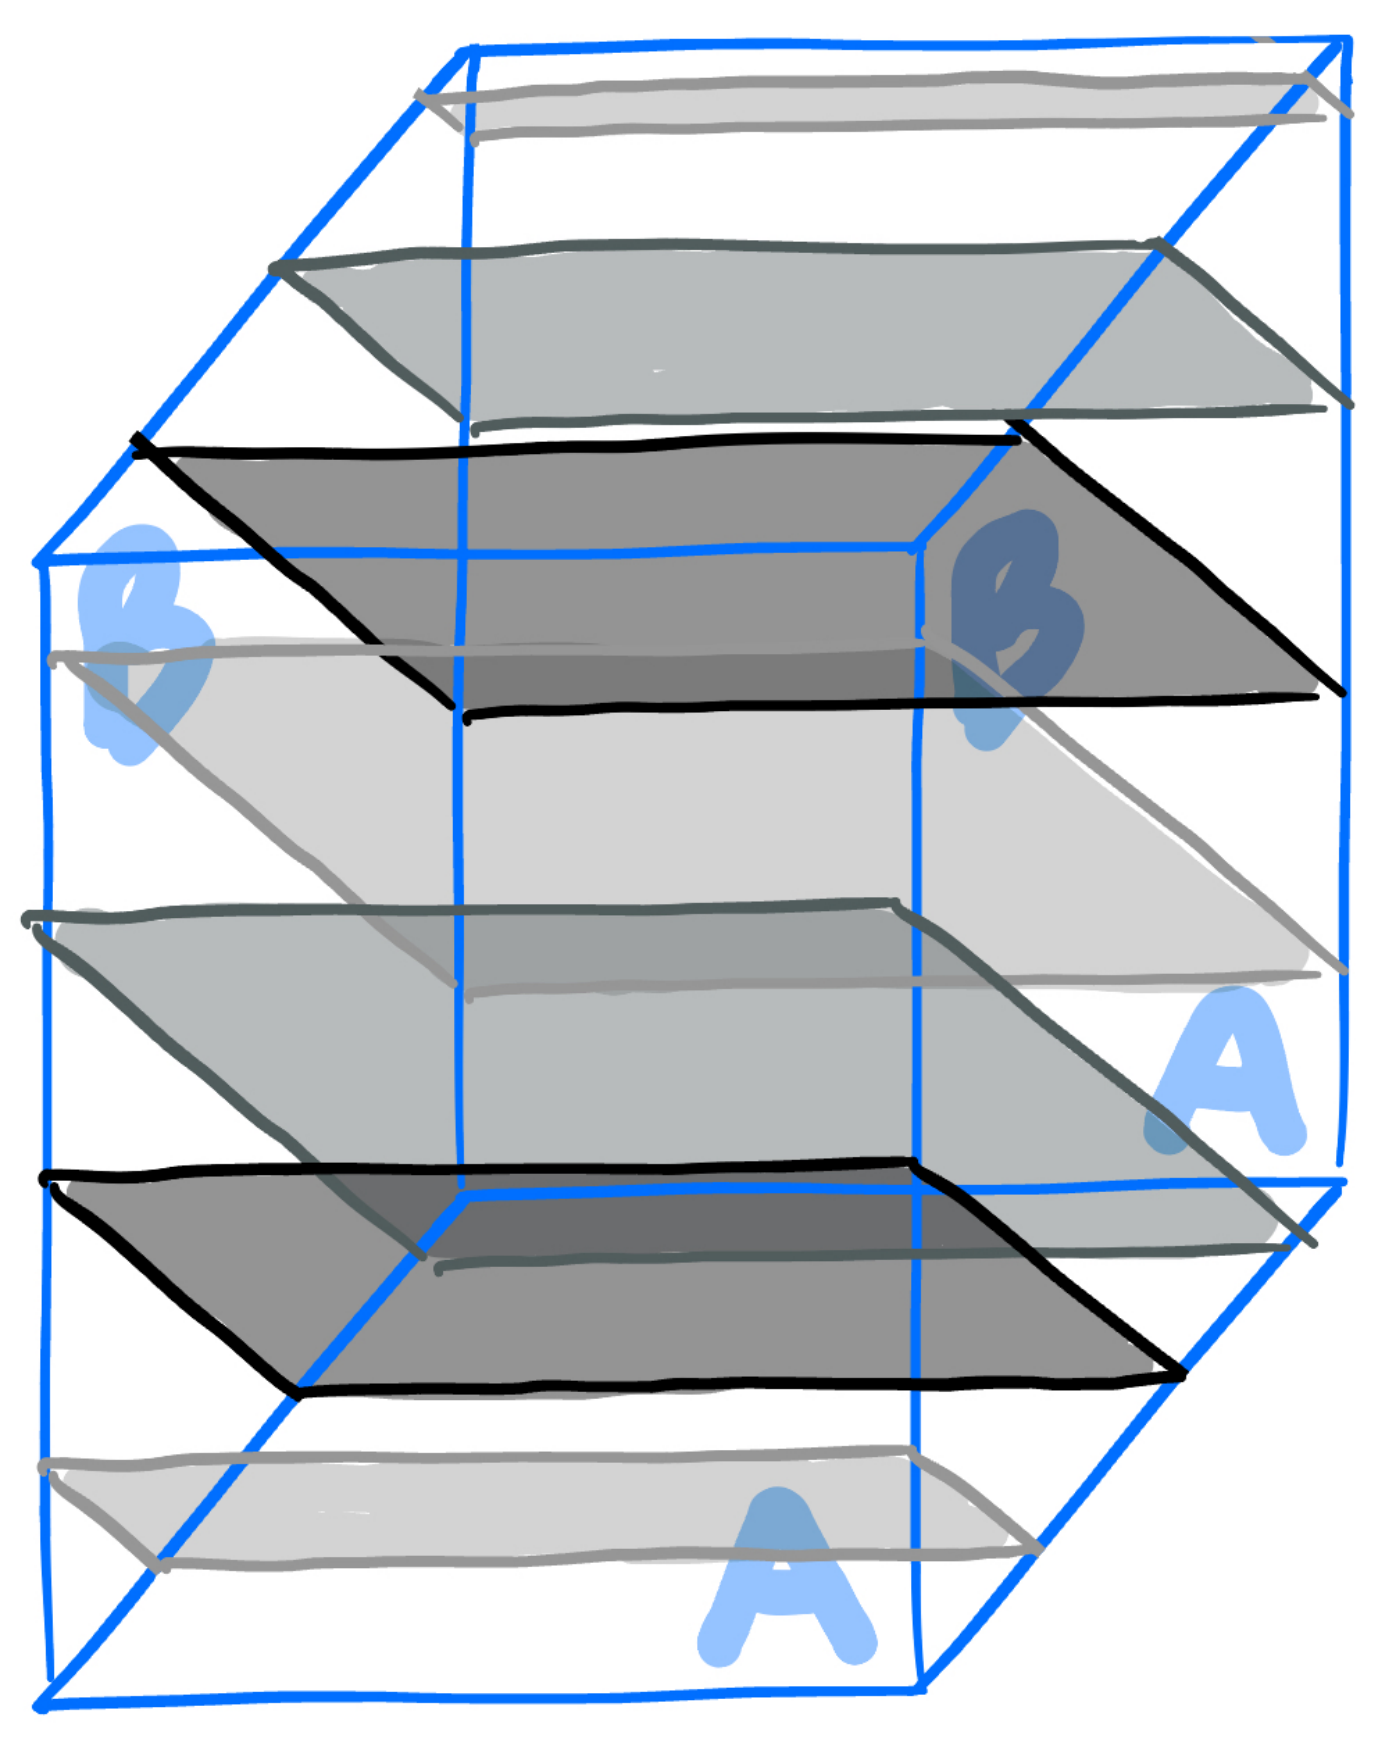
\includegraphics[width=100pt]{figures/qubits/floquetifying/colour_code/spacetime_volumes/toric}
\end{aligned}
\end{equation}

So it's impossible to interpret these as timeslices in a new code, because time can't run in a circle!
A possible alternative strategy in the case that we're given a code that lives on a torus is the following:
one can first try to Floquetify a suitably sized subdiagram of the bulk, then try to impose periodic boundary conditions on the resulting Floquetified diagram,
and see whether the desired error correction properties carry over -- number of encoded logical qubits, distance, etc.

Let's apply this strategy to the Floquetified subdiagram on the right hand side of \Cref{fig:floquetified_colour_code_measurement_schedule}.
Suppose we take the wonky rectangle in that figure and tile copies of them to create a large ZX-diagram.
Let the measurements represented by this ZX-diagram be those of the bulk of a new Floquet code at time $0$.
Define the measurements at subsequent timesteps $t+1$ according to the rules given in the last subsection -- namely, translate the measurements from time $t$ by $(-1, -3)$.
Then impose toric boundary conditions on this large diagram: this is our new Floquet code.

It turns out that we can't just tile the torus any way we like with these rectangles;
in order to actually encode any logical information,
we must choose a tiling in which the number of columns of such rectangles is a multiple of three.
That is, if we choose a tiling in which this is not the case,
then we find that the logical Pauli group $\lpg{t}$ becomes trivial after a full period of 13 measurement rounds
(we calculated this using Stim's stabilizer group functionality).
When we choose a tiling in which it is the case, on the other hand,
we find that $\lpg{t} \cong \PPP_4$ after establishment, just as for the toric colour code.
One explanation for this is that the wonky rectangle of \Cref{fig:floquetified_colour_code_measurement_schedule} corresponds to a thin non-three-face-colourable strip of the original colour code, as shown in \Cref{fig:floquetified_toric_colour_code_tile}.
So trying to define the new code on a wonky rectangle with toric boundary conditions is analogous to trying to define a colour code on a non-three-face-colourable toric graph.
The latter is known to encode no qubits, so it makes sense that the former does too.
On the other hand, if we first tile together three wonky rectangles and then impose periodic boundaries, this is analogous to taking a slightly thicker three-face-colourable strip of colour code and imposing periodic boundaries, as shown in \Cref{fig:floquetified_toric_colour_three_tiles}.
Since the latter does encode the usual four logical qubits, it again makes sense that the former does too.

\begin{figure}[p]
    \centering
    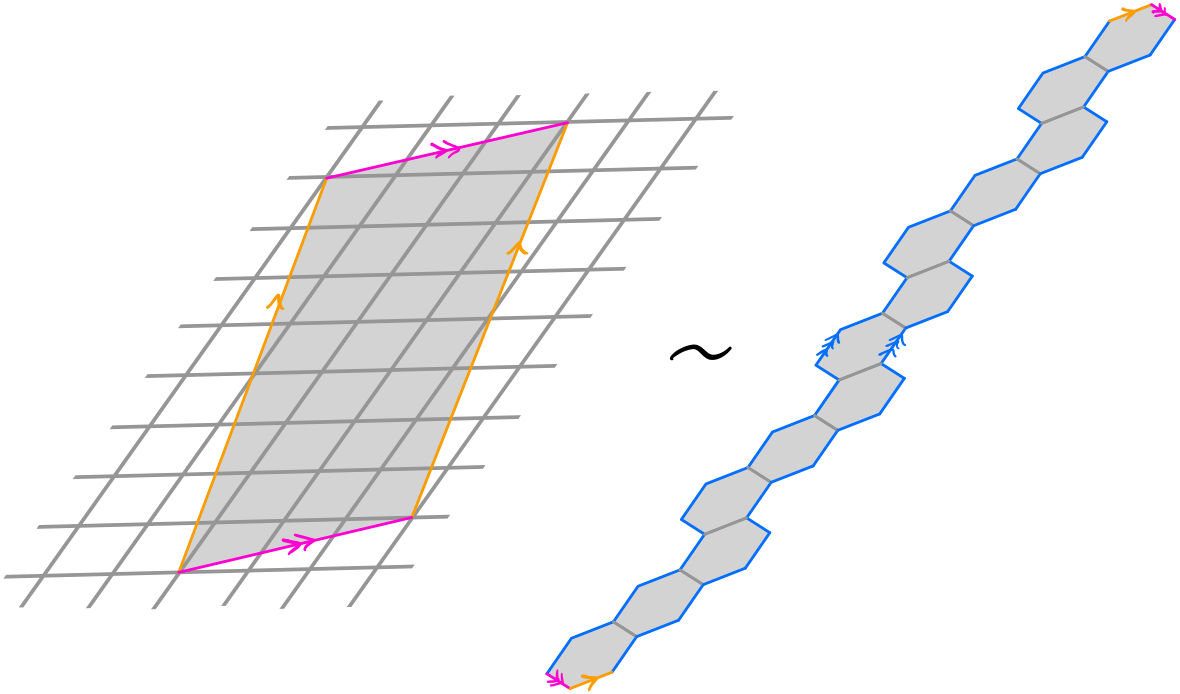
\includegraphics[width=350pt]{figures/qubits/floquetifying/colour_code/floquetified/toric/one_tile}
    \caption{%
        Imposing periodic boundary conditions on a single rectangle of the Floquetified colour code bulk,
        as in \Cref{fig:floquetified_colour_code_measurement_schedule},
        defines a Floquet code with no logical qubits.
        As a patch of the Floquetified colour code bulk,
        this rectangle corresponds to the strip of colour code bulk on the right.
        Since this strip is not three-colourable,
        imposing toric boundary conditions on it prevents it from supporting a colour code.}
    \label{fig:floquetified_toric_colour_code_tile}
\end{figure}

\begin{figure}[p]
    \centering
    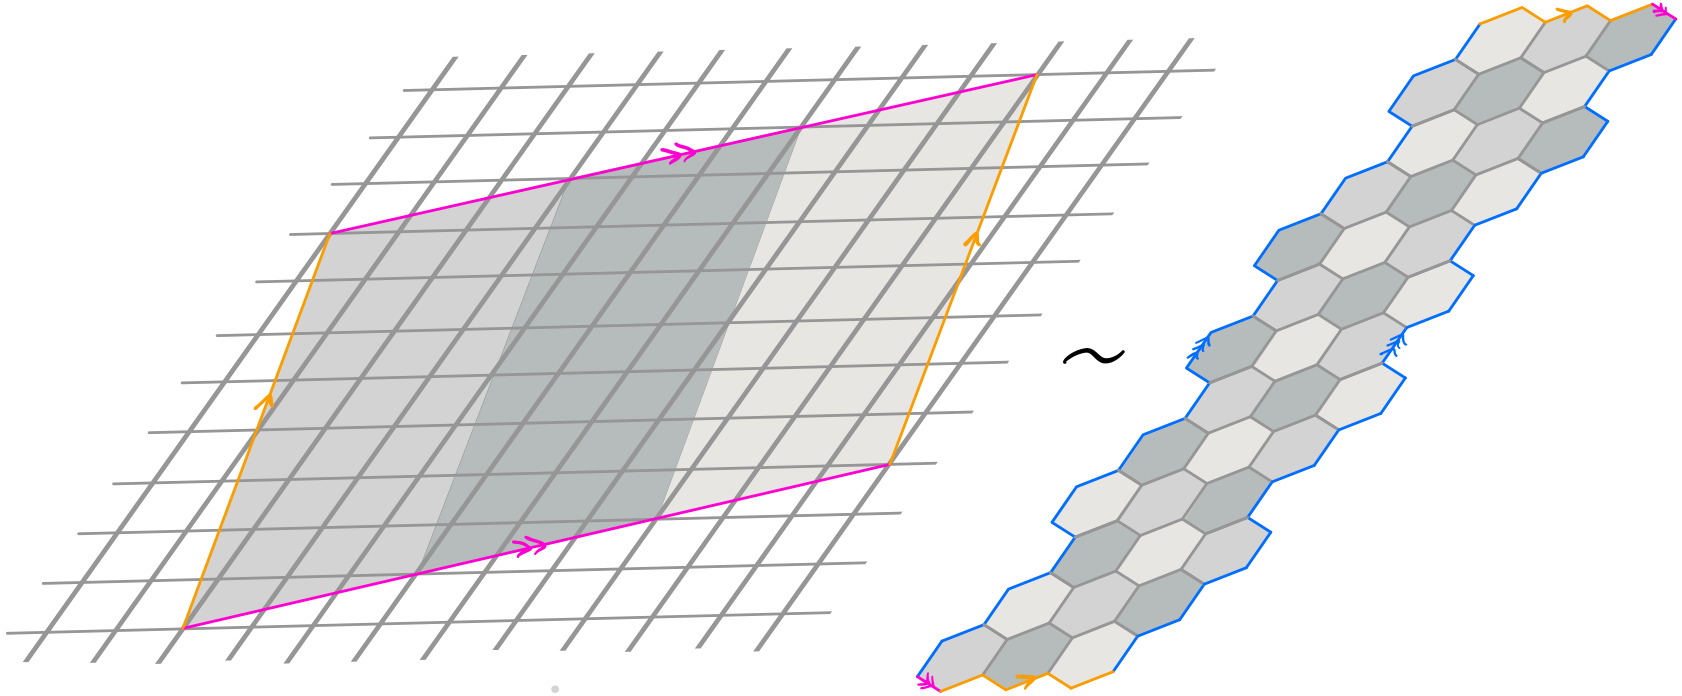
\includegraphics[width=\linewidth]{figures/qubits/floquetifying/colour_code/floquetified/toric/three_tiles}
    \caption{%
        If we instead tile together a multiple of three columns of these rectangles,
        we define a Floquet code with four logical qubits -
        the same number as for the toric colour code.
        The left diagram of this figure is thus the support of
        the smallest member of our family of toric Floquetified colour codes.
        As a patch of the Floquetified colour code bulk,
        this corresponds to the wider strip of colour code bulk on the right.
        Unlike in \Cref{fig:floquetified_toric_colour_code_tile}, this strip is three-colourable,
        and thus supports a colour code when toric boundary conditions are imposed on it.}
    \label{fig:floquetified_toric_colour_three_tiles}
\end{figure}


%While this works for the colour code (see next subsection),
%it's very ad-hoc - it would be nice to know if there are any guarantees that such a method will always work.

%The Floquetification process described above can be applied directly to planar colour codes,
%and will lead to a new code that is itself planar.
%But since the boundaries of the original code look different to the bulk,
%extra work needs to be done to Floquetify these correctly.
%Furthermore, the resulting Floquet code can exhibit a `drifting' behaviour,
%which we discuss in more detail in \Cref{subsec:drift}.
%There are potential perks of this behaviour - e.g.\ for removing leakage -
%but it's also handy to have a code that doesn't drift.
%One might think we could get around these two issues by starting with the colour code defined on a torus,
%which has no boundaries to worry about.
%But viewing our procedure as tilting the time direction in a ZX-diagram for a code,
%as described in the last section,
%we find we can only give well-defined new timesteps when the code we start with is planar -
%this is discussed in more depth in \Cref{subsec:periodic_boundaries}.
%Instead, if we want to avoid boundaries,
%what we can do is Floquetify only the bulk,
%which will give the bulk of a potential new Floquet code,
%then see if placing this new bulk on a torus still encodes logical qubits.
%In \Cref{subsec:colour_code} we apply the two ideas described above -
%we Floquetify a planar colour code,
%and place the Floquetified colour code bulk from this section on a torus.

%In this section, we expand on what we mean by a code exhibiting \textit{drift},
%and sketch some ideas as to how it might be avoided.
%Then we describe what goes wrong when attempting to Floquetify a non-planar code,
%before turning our attention back to our specific example of the colour code.

\subsection{Beyond the bulk: planar boundaries}\label{subsec:drift}

The second option to avoid making time run in a circle is to restrict ourselves to Floquetifying planar codes.
If we do this using the idea of reinterpreting the time direction, the resulting Floquet code will exhibit \textit{drift}.
This is the property whereby at any timestep $t$, new qubits might need to be initialised and entangled into the code,
or old qubits might be measured out and not used again.
If these new qubits being entangled in are always on one boundary of the code, with the old qubits being measured out always on the opposite boundary, and the code is being implemented on hardware that requires qubits to be in fixed positions (e.g.\ on a superconducting chip), the code will appear to slowly `drift' across the hardware in the direction of the new qubits.
For example, if the qubits of the code roughly form a square,
and qubits on the top boundary of this square are being regularly measured out,
while on the bottom boundary new qubits are regularly being entangled in,
then the code as a whole will seem to drift downwards.
We show this process on the left hand side of \Cref{fig:drifting_spacetime_volume}.

\begin{figure}[b]
    \centering
    
\includegraphics[width=\linewidth]{figures/qubits/floquetifying/colour_code/spacetime_volumes/drift}
    \caption{%
        Here blue prisms represent ZX-diagrams of codes,
        while grey planes are timeslices $t_0 < t_1 < t_2$ after the time direction has been tilted.
        The shaded grey squares show the intersection of the code's ZX-diagram with a particular timestep.
        On the left, we see that taking a stabilizer code
        and tilting the time direction to get an equivalent Floquet code naturally causes drift -
        notice how the shaded grey intersections change position within the timeslices $t_0$, $t_1$ and $t_2$.
        On the right, we show that one way to avoid drifting boundaries is to Floquetify a code that is itself moving;
        here the grey intersections are always in the same place within the timeslices $t_0$, $t_1$ and $t_2$.}
    \label{fig:drifting_spacetime_volume}
\end{figure}

There are some perks that come with a drifting code.
The main one is preventing leakage -- if the whole code is drifting and all qubits get measured out eventually then leakage cannot build up too badly, in the way that it can if we have a fixed set of data qubits that are only measured out at the very end of the logical computation.
But obviously there are drawbacks too -- chiefly that if your hardware does involve a chip of fixed qubits then at some point your code is going to drift all the way to the edge of your chip!
So it's worth thinking about how we might avoid drift.

In fact, we saw one way already,
when we Floquetified the $\qcode{4, 2, 2}$ code in \Cref{sec:floquetifying_422}.
Ordinarily, the resulting code would exhibit drift,
in exactly the fashion visualised on the left hand side of \Cref{fig:drifting_spacetime_volume}.
However, our Floquetification re-used qubits cyclically;
once the pair of qubits on the top boundary of the code were measured out,
they were immediately re-entangled into the bottom boundary of the code at the next timestep -
see the rightmost diagram of \Cref{fig:4_2_2_rewritten}.
In this sense, we made our code drift around in a circle, which gives it its double hexagon shape.
While this works nicely for the very small $\qcode{4, 2, 2}$ code,
it's not a good general solution from a practical perspective,
since for hardware with qubits in fixed positions,
an unusual connectivity would be required in order to implement a large code that drifts circularly.
(For other types of hardware, where qubits can be moved around and re-used,
this would be less of a problem).

Another potential solution is to Floquetify a code that is already moving,
so as to cancel out the drift that results from Floquetifying it.
For example, the rotated surface code can be grown outwards from one boundary (the top one, say),
then contracted from the opposite one (the bottom),
such that it appears to move in a particular direction (upwards) -
see, for example, \Ccite[Figure 40(c)]{GameOfSurfaceCodes}.
The same idea can be used to move other stabilizer and subsystem codes.
If such a code can be moved in an appropriate direction and at an appropriate speed,
the resulting Floquetification will remain put;
this is sketched abstractly on the right hand side of \Cref{fig:drifting_spacetime_volume}.

Other systematic ways one might hope to obtain non-drifting boundaries involve changing the operation schedule.
Suppose a drifting Floquetification has schedule
$\OOO = (\OOO_0, \OOO_1, \ldots, \OOO_{T})$.
Consider a new Floquet code with schedule
$\OOO = (\OOO_0, \OOO_1, \ldots, \OOO_{T}, \OOO_{T}, \OOO_{T-1}, \ldots, \OOO_0)$.
This new code would drift in one direction in timesteps $0 \leq t < T$,
but then drift in exactly the opposite direction in timesteps $T \leq t < 2T$,
and so overall it would stay within a bounded region,
while still having the required error correcting properties.

Let's apply this approach to the colour code.
Consider a planar colour code defined on a parallelogram; we show one timeslice of the measurements in this code on the left hand side of \Cref{fig:floquetified_planar_colour_code_zx_rewritten}.
On the right hand side, we show the Floquetified version of this timeslice.
We can repeat this for multiple rounds of measurements to get a Floquetified version of this code;
this is shown in \Cref{fig:floquetified_planar_colour_code_zx}.

%Option one is to Floquetify a planar colour code, which will give us a Floquet code with drifting boundaries.
%We show this explicitly in
%\Cref{fig:floquetified_planar_colour_code_zx_rewritten,fig:floquetified_planar_colour_code_drift,fig:floquetified_planar_colour_code_zx}
%below, for a small colour code that lives on a parallelogram,
%but the idea extends to a planar colour code of any size.

\begin{figure}[btp]
    \centering
    
\includegraphics[width=\linewidth]{figures/qubits/floquetifying/colour_code/floquetified/planar/zx_rewritten}
    \caption{%
        Two equivalent ZX-diagrams for one round of a small planar colour code on a parallelogram,
        in which all $Z \otimes Z \otimes \ldots \otimes Z$ measurements are performed.
        As in \Cref{fig:colour_code_rewritten}, the grey highlighted bars have no meaning in the ZX-calculus,
        and instead denote timesteps of the corresponding Floquetified code.}
    \label{fig:floquetified_planar_colour_code_zx_rewritten}
\end{figure}

\begin{figure}[htbp]
    \centering
    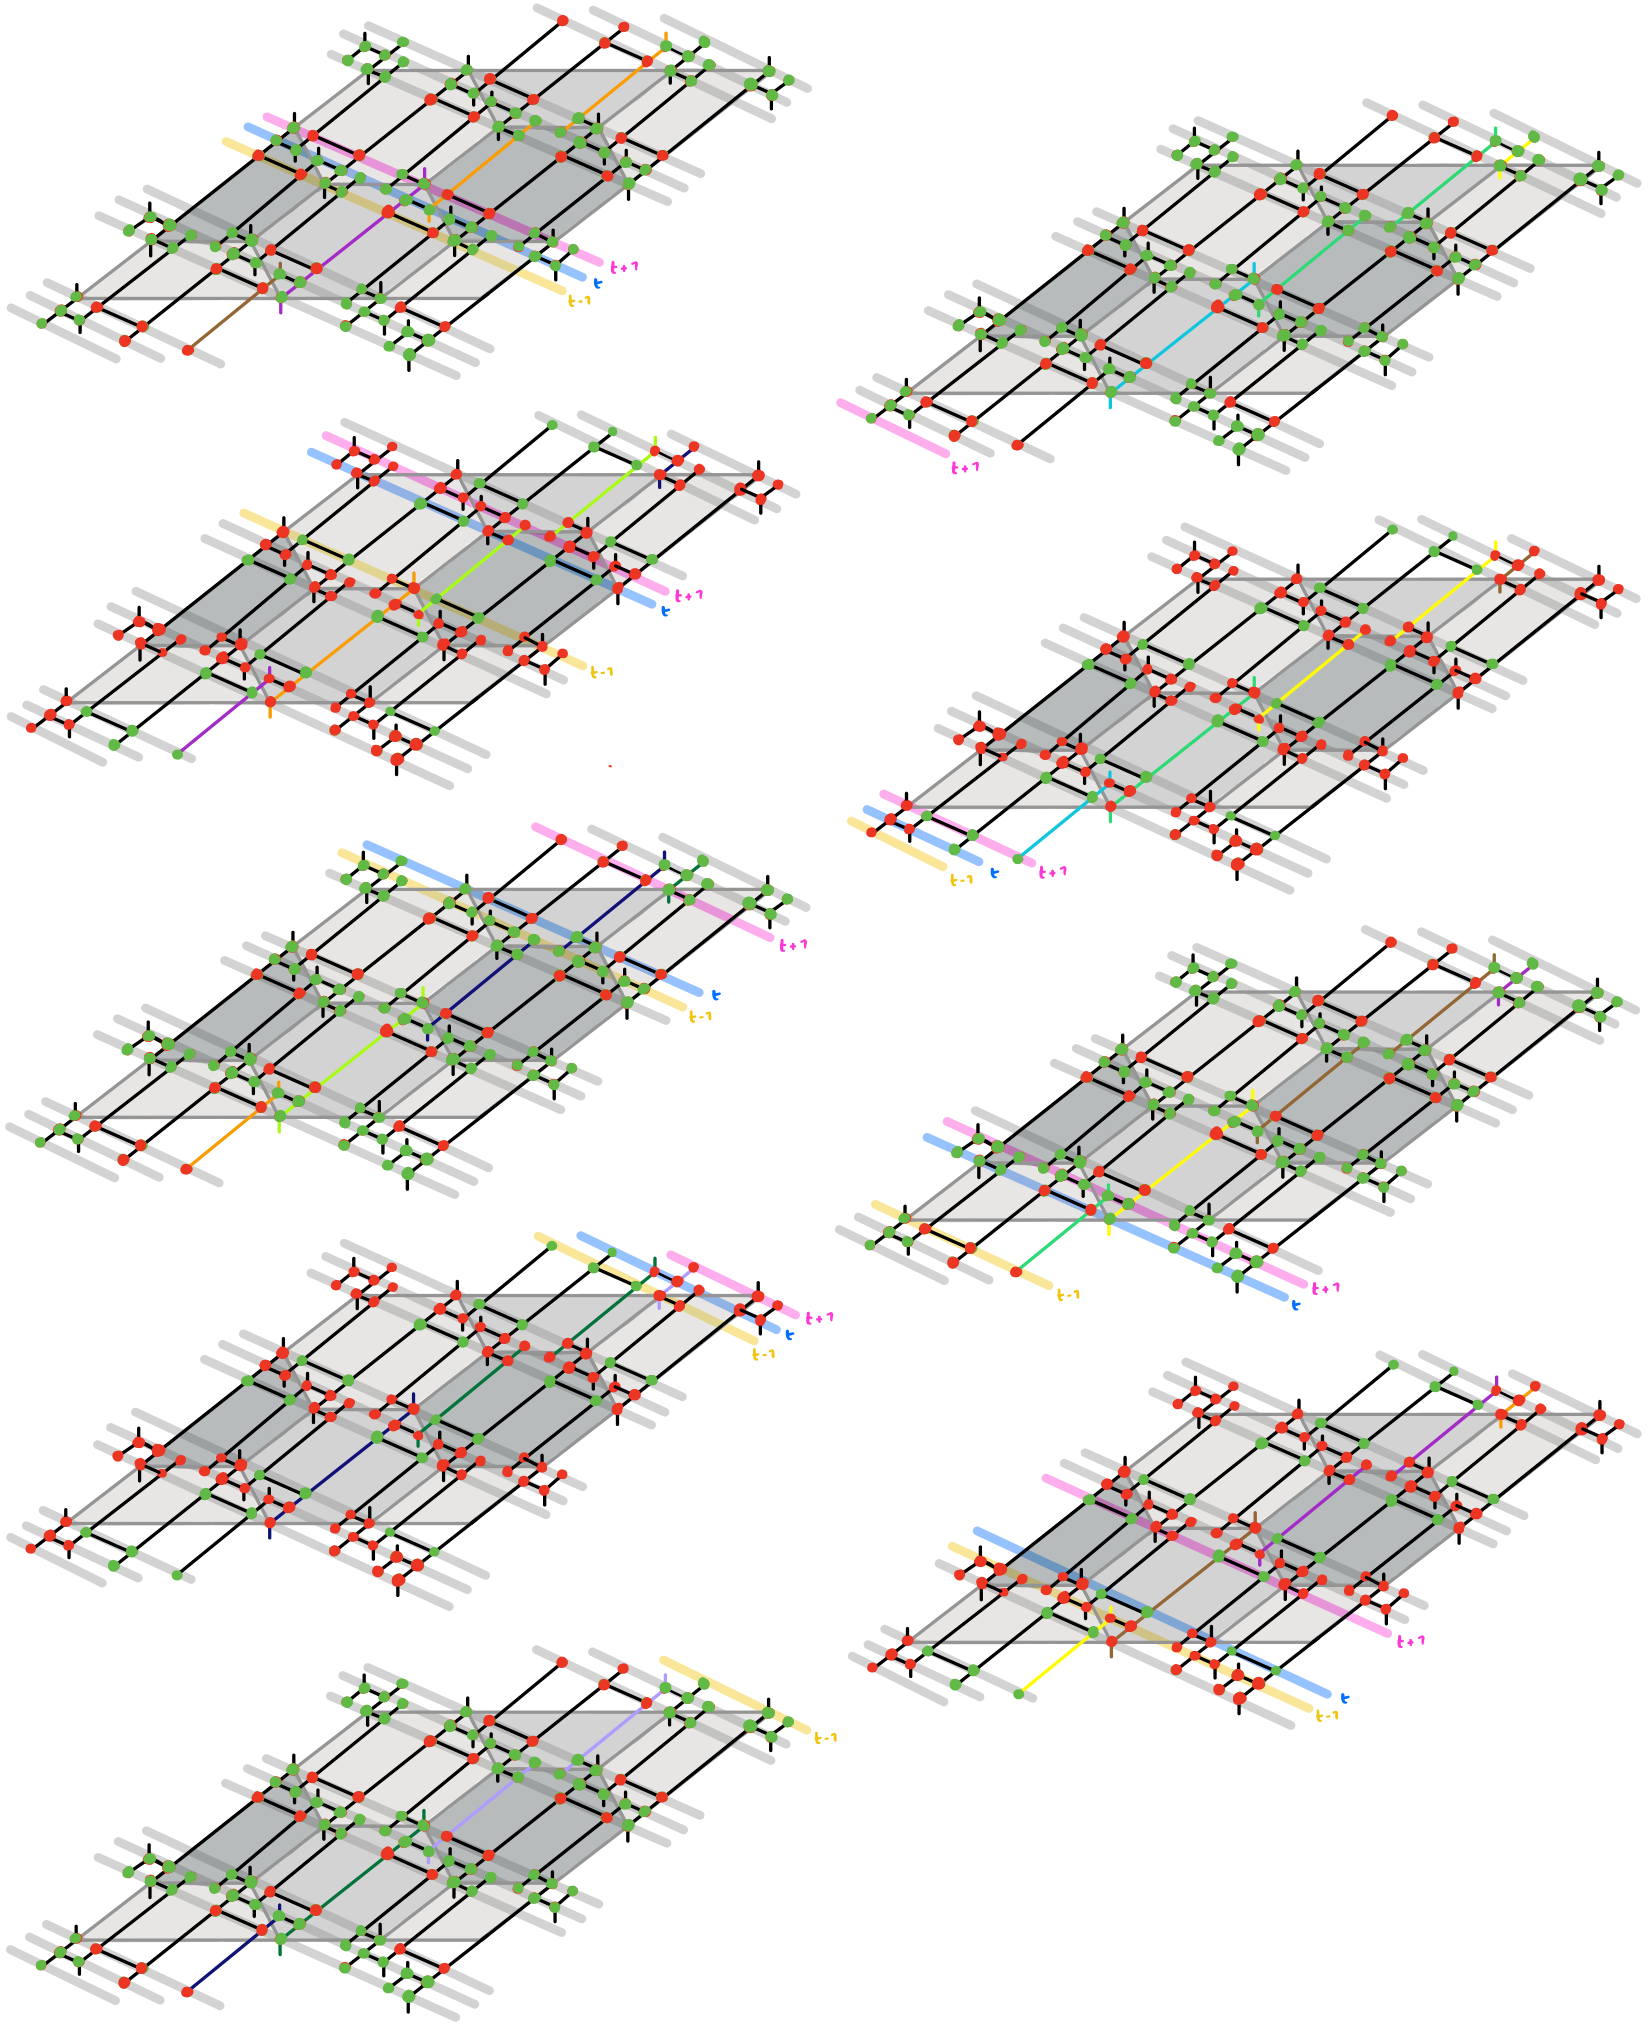
\includegraphics[width=\linewidth]{figures/qubits/floquetifying/colour_code/floquetified/planar/zx_multiple_timesteps}
    \caption{%
        ZX-diagram of nine rounds of the planar colour code.
        This figure should be read columnwise up the page; first the left column, then the right.
        Much like in \Cref{fig:colour_code_rewritten},
        vertical ZX-wires between consecutive layers have been omitted for clarity.
        Instead we state in words that, for a vertex $v$ of the underlying honeycomb lattice,
        the small vertical upwards wire closest to $v$ going upwards from one layer
        is connected to the small vertical wire closest to $v$ protruding downwards from the next layer.
        Certain wires have been coloured - these indicate the world-lines of different qubits.
        Specifically, these are the world-lines of qubits that in a single column
        on the square lattice of the Floquetified code,
        as denoted by coloured crosses in \Cref{fig:floquetified_planar_colour_code_drift}.
        Grey highlighted bars again denote timesteps of the Floquetified code;
        three of them have been coloured yellow, blue and pink respectively,
        denoting three consecutive timesteps $t-1$, $t$ and $t+1$.}
    \label{fig:floquetified_planar_colour_code_zx}
\end{figure}

The sequence of measurements that a particular qubit undergoes
will be almost the same as that described in \Cref{sec:floquetifying_colour_code},
with the exception that qubits near a boundary can be measured out earlier or initialised later than usual.
Additionally, as a consequence, a pairwise measurement that would ordinarily have been performed is omitted
if one of the two qubits it would have applied to has been measured out early or initialised late.
Detectors and logicals can again be found via Pauli webs,
by drawing them on the ZX-diagram for the planar colour code and seeing how they map to the Floquetification.
In the bulk, they will look as described in \Cref{sec:floquetifying_colour_code}.

\begin{figure}[htbp]
    \centering
    \hspace{50pt}
    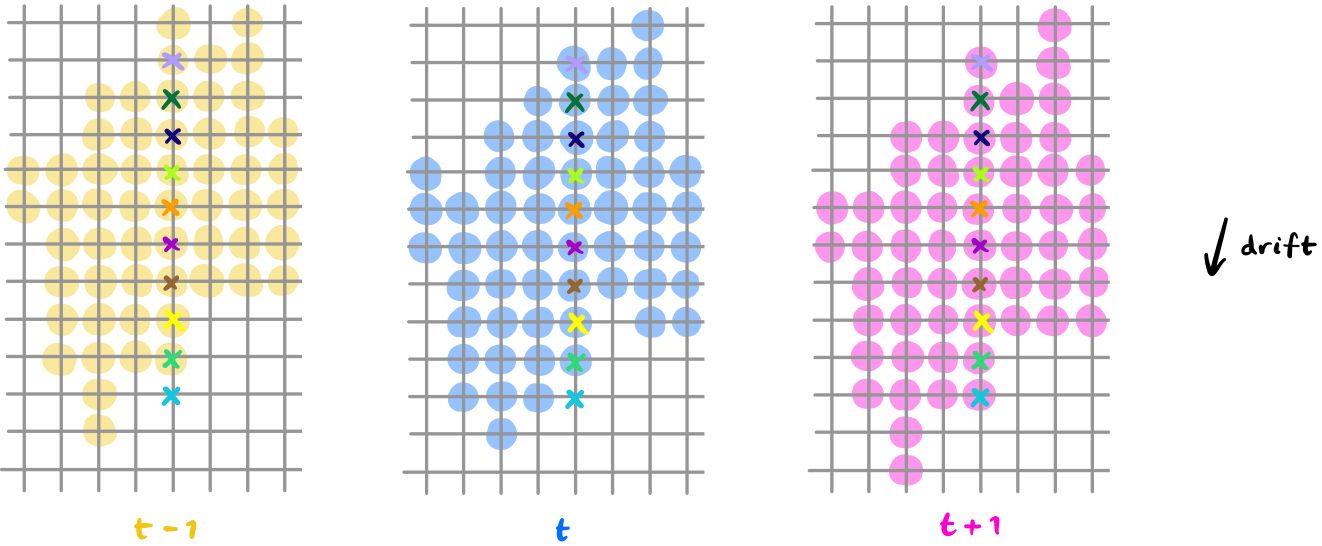
\includegraphics[width=\linewidth]{figures/qubits/floquetifying/colour_code/floquetified/planar/drift}
    \caption{%
        The square lattice layout of the Floquetified planar colour code, with qubits on vertices,
        at consecutive timesteps $t-1$, $t$ and $t+1$.
        Vertices marked with a coloured cross correspond to
        qubit world-lines of the same colour in \Cref{fig:floquetified_planar_colour_code_zx}.
        Vertices highlighted yellow, blue or pink are \textit{active} at the respective timestep $t-1$, $t$ or $t+1$.
        Here \textit{active} means the qubit is initialised for the first time on or before this timestep,
        and is measured out for the last time on or after this timestep.
        If we were to plot the active qubits across all timesteps,
        we would see that the code drifts downwards and slightly to the left.}
    \label{fig:floquetified_planar_colour_code_drift}
\end{figure}

As things stand, this Floquetified code will exhibit drift, as shown in \Cref{fig:floquetified_planar_colour_code_drift}.
If we wish to prevent it from drifting,
we could instead force our parallelogrammatic colour code to regularly
expand outwards from its top and right boundaries,
and contract inwards from its bottom and left boundaries,
such that this cancels out the drift that results from Floquetifying it.
The expansion is performed by preparing pairs of qubits in Bell states,
then entangling them into the code by measuring the stabilizers of a bigger colour code.
Similarly, contraction is done by measuring out pairs of qubits in the Bell basis.
We must be a little careful here to maintain the code's timelike distance;
when measuring the stabilizers of the new, bigger code during an expansion phase,
we must repeatedly measure these stabilizers for $d$ rounds, where $d$ is the distance of the original code.
Contraction, however, can be done instantaneously.
The distance by which we need to expand is determined by how fast the world-lines of qubits in the Floquetified code
move forwards and rightwards through the ZX-diagram for the underlying colour code,
as in \Cref{fig:floquetified_planar_colour_code_zx} or the right hand side of \Cref{fig:colour_code_rewritten}.
%for a reminder of what this looks like.
Let \textit{rows} and \textit{columns} in the honeycomb lattice be defined as
the pink and orange lines respectively in the following diagram:

\begin{equation}\label{eq:honeycomb_rows_columns}
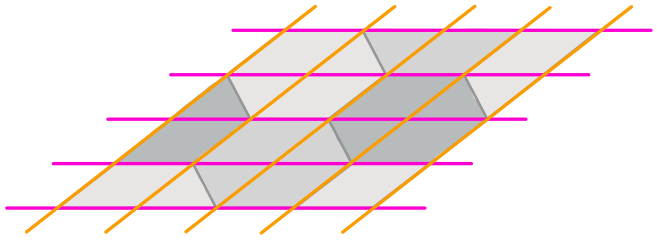
\includegraphics[width=200pt, valign=c]{figures/qubits/floquetifying/colour_code/rows_columns}
\end{equation}


\begin{figure}[p]
    \centering
    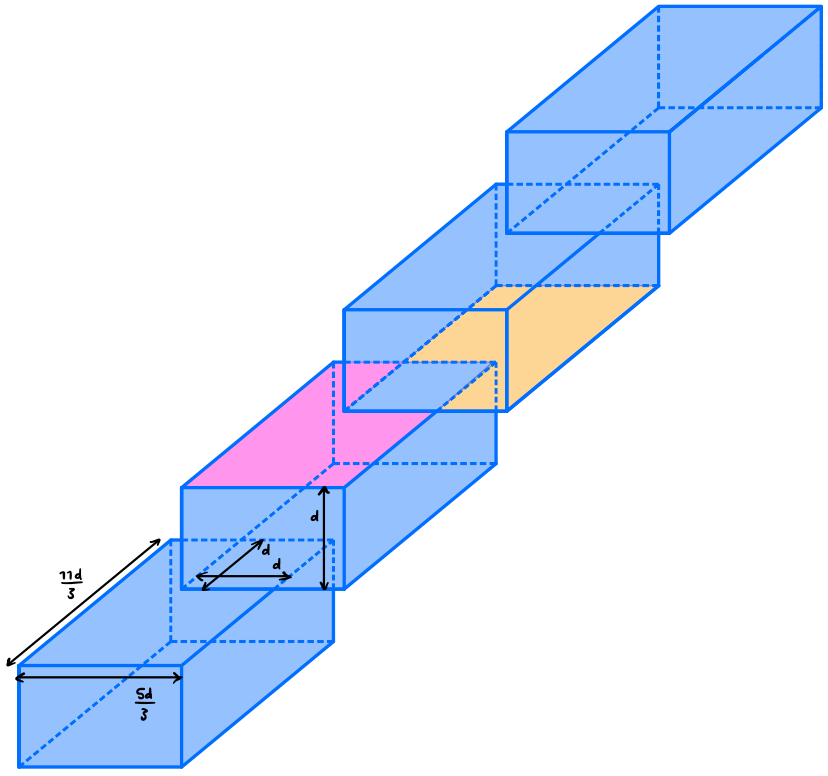
\includegraphics[width=250pt]{figures/qubits/floquetifying/colour_code/floquetified/planar/cancelling_drift}
    \caption{%
        An abstraction of a ZX-diagram of a parallelogrammatic colour code
        which expands and contracts in the fashion specified in the text.
        In this figure, time goes directly upwards.
        The distance of the original colour code is denoted $d$.
        Two timelike boundaries are shaded;
        at the pink one, pairs of qubits are measured in the Bell basis,
        while at the orange one, Bell pairs are entangled into the code.}
    \label{fig:floquetified_planar_colour_code_cancelling_drift}
\end{figure}

\begin{figure}[p]
    \centering
    \begin{subfigure}{\textwidth}
        \centering
        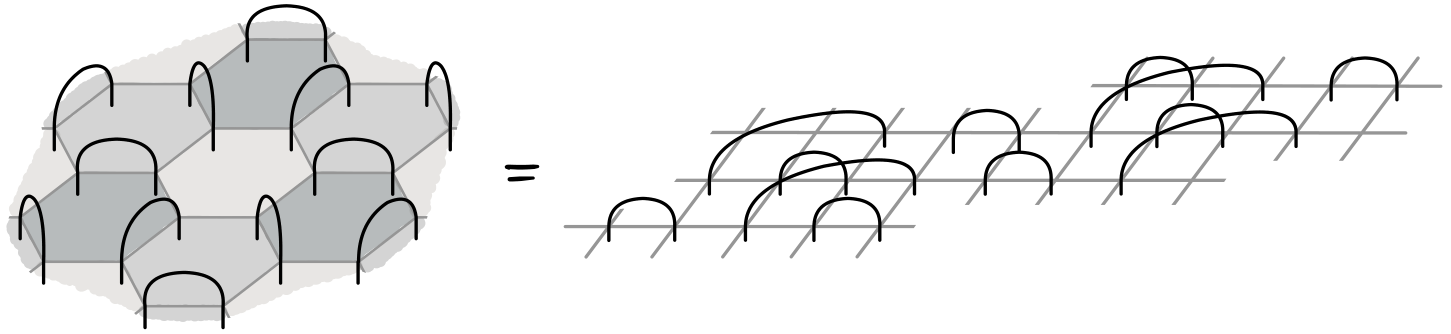
\includegraphics[width=0.9\textwidth, valign=c]{figures/qubits/floquetifying/colour_code/floquetified/planar/timelike_boundaries/measuring_out}
        \caption{\ }
        \label{fig:floquetified_planar_colour_code_measuring_out}
    \end{subfigure}
    \begin{subfigure}{0.15\textwidth}
        \centering
        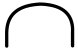
\includegraphics[width=30pt, valign=c]{figures/qubits/floquetifying/colour_code/floquetified/planar/timelike_boundaries/destructive_bell_measurement}
        \caption{\ }
        \label{fig:floquetified_planar_colour_code_destructive_bell_measurement}
    \end{subfigure}
    \begin{subfigure}{0.15\textwidth}
        \centering
        
\includegraphics[width=30pt, valign=c]{figures/qubits/floquetifying/colour_code/floquetified/planar/timelike_boundaries/non_destructive_bell_measurement}
        \caption{\ }
        \label{fig:floquetified_planar_colour_code_non_destructive_bell_measurement}
    \end{subfigure}
    \begin{subfigure}{0.6\textwidth}
        \centering
        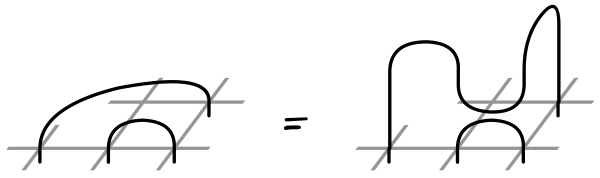
\includegraphics[width=200pt, valign=c]{figures/qubits/floquetifying/colour_code/floquetified/planar/timelike_boundaries/local_circuit}
        \caption{\ }
        \label{fig:floquetified_planar_colour_code_local_readout_circuit}
    \end{subfigure}
    \caption{
        \textbf{(a)}
        The Bell basis measurements on a timelike boundary of the colour code,
        such as the pink one in \Cref{fig:floquetified_planar_colour_code_cancelling_drift},
        and their image in the square lattice Floquetification.
        \textbf{(b)}
        A destructive Bell basis measurement (or rather, post-selection) in the ZX-calculus.
        \textbf{(c)}
        A non-destructive Bell basis measurement (or rather, post-selection) in the ZX-calculus.
        \textbf{(d)}
        Two equivalent ZX-diagrams for performing a pair of Bell basis measurements on four qubits.
        Whereas the diagram on the left involves a measurement between two non-neighbouring qubits on the square lattice,
        the diagram on the right respects this connectivity constraint,
        but costs one extra Bell basis measurement.
    }
    \label{fig:floquetified_planar_colour_code_timelike_boundaries}
\end{figure}

Suppose we now have a parallelogrammatic colour code with algebraic distance $d$.
The geometry of the parallelogram forces $d$ to be even.
Such a code occupies $\frac{3d}{2} - 1$ rows and $\frac{3d}{2} - 1$ columns in the honeycomb lattice.
%and vice versa.
After every $d$ rounds of stabilizer measurements,
the code needs to have moved $4d$ rows forwards and $d$ columns rightwards in the honeycomb lattice
in order to cancel out the drift the Floquetification process would bring.
It's most convenient to expand and contract the colour code by multiples of $3$ rows or columns,
so let's also assume that $d$ is an even multiple of $3$.
Thus, during an expansion phase, the code occupies $\frac{3d}{2} - 1 + 4d$ rows and $\frac{3d}{2} - 1 + d$ columns.
The distance of the code during such a phase is therefore
$\frac{11d}{3}$ in the forwards direction and $\frac{5d}{3}$ in the rightwards direction.
We sketch this in \Cref{fig:floquetified_planar_colour_code_cancelling_drift}.

The extra complication that this idea entails is that we now have also timelike boundaries to Floquetify.
These are points at which pairs of qubits either become Bell states and get entangled into the code,
or get measured out in the Bell basis.
We could just do the same thing in our Floquetified code, but while the pairs of qubits to be entangled/measured
are all neighbours in the honeycomb lattice, they are not all neighbours in the square lattice of the Floquetified code.
This is shown in \Cref{fig:floquetified_planar_colour_code_measuring_out}.
Fortunately, as shown in that \Cref{fig:floquetified_planar_colour_code_local_readout_circuit},
we can construct a circuit on groups of four qubits which achieves the same thing
but respects the nearest neighbour connectivity of the square lattice.
